
\section{Free-space Optics}
\label{sec:fso}

The purpose of the trials with the free-space optical (FSO) links was to
ascertain the extent to which fog, a common feature of the Scottish
environment especially in coastal areas, would affect their
use. Obviously fog would attenuate the signal to some extent since
the units operate in the near-infrared or visible spectrum -- which is
affected by clouds but to a lesser extent than shorter wavelengths --
but we were interested in finding out if their operational window was,
on average, large enough to justify the considerable expense.
\begin{figure}
  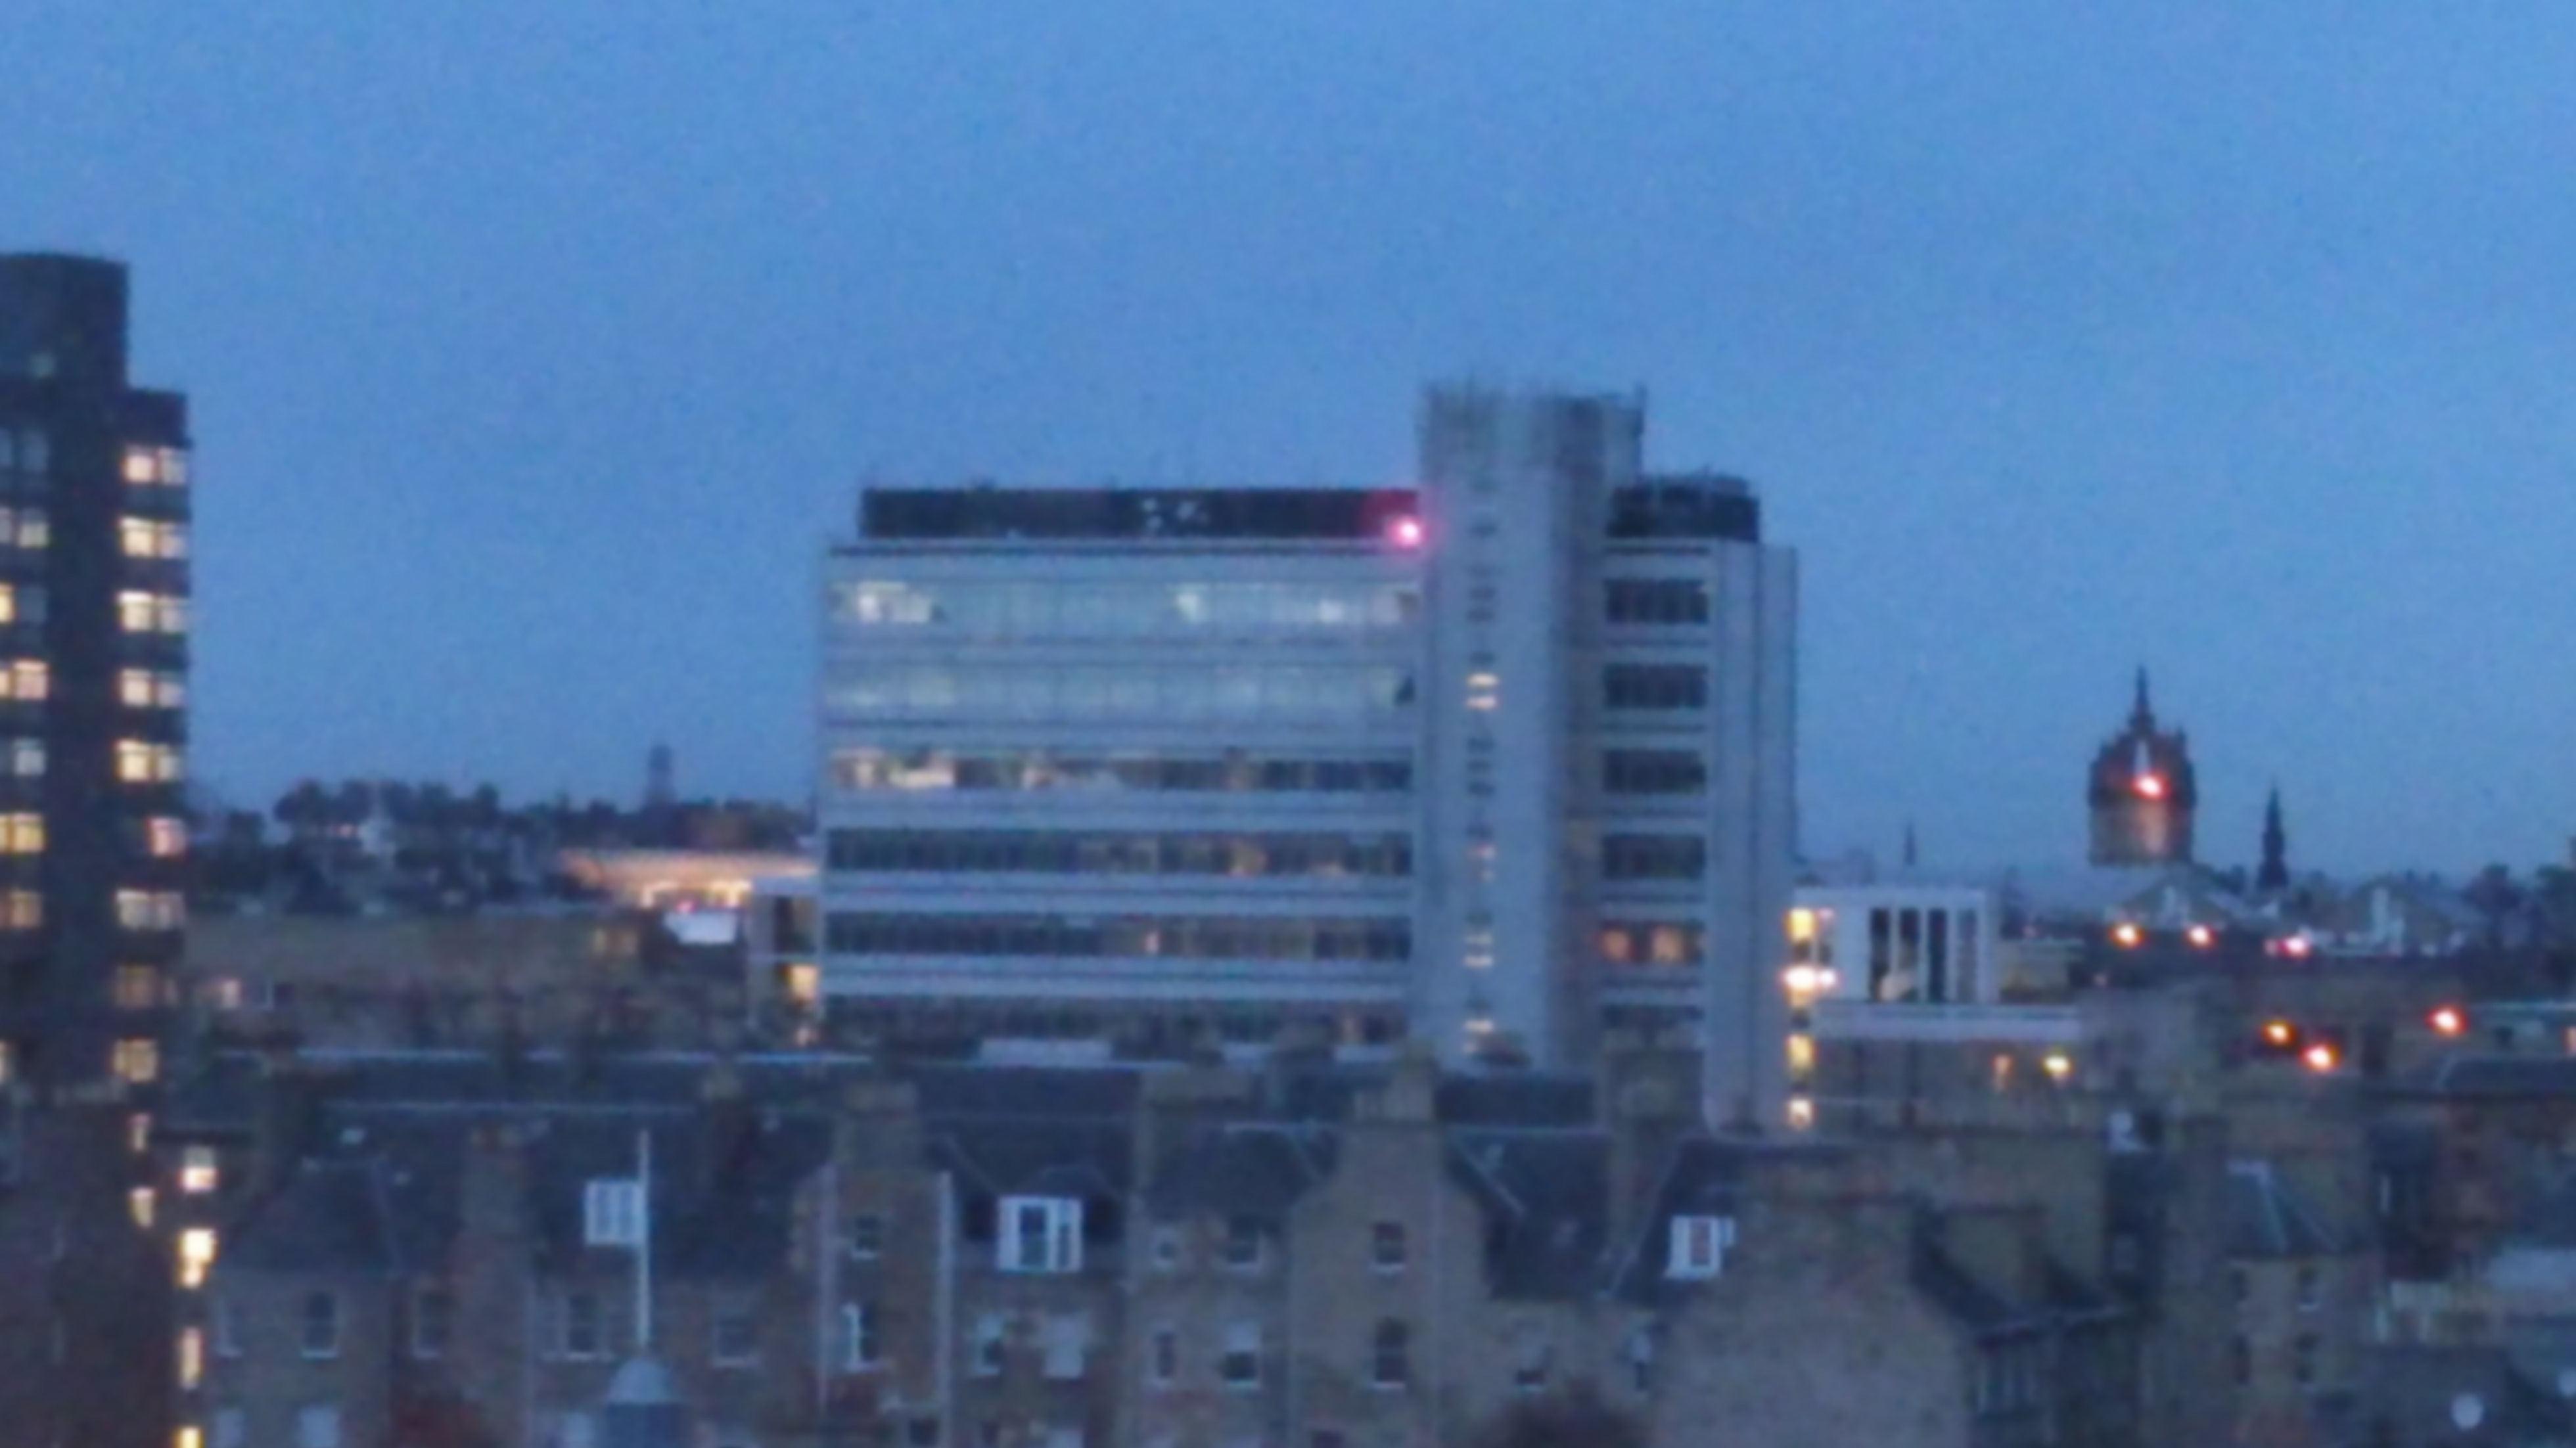
\includegraphics[width=\textwidth]{at-laser.jpg}
\end{figure}

The Scottish Government had a preferred vendor, CableFree, for the
equipment though we were formally free to select another. Our budget
was only about \pounds 10,000 for the equipment. The FSO vendors that
are well-regarded in industry such as F-Sona and Canon do not produce
anything in this price range. Small wonder as their primary market is
the military -- optical links are much harder to eavesdrop upon
compared to radio links. Two vendors were within our price range:
Geodesy of Hungary and Cablefree.

We selected the suggested vendor partly because they were a local
(i.e. UK-based) company on the theory that they might be more
responsive and accessible. We were also given to believe -- with no
evidence -- that their Hungarian competitor used inferior, older
technology. It is difficult to tell the extent to which this was
true without comparing the equipment from both manufacturers side by
side. We were subjected to the hard-sell and given very little
concrete information without signing non-disclosure agreements that
would prevent our conducting any useful research. As it was, not
executing the NDAs prevented us from properly instrumenting the
equipment and measuring its behaviour at any but very coarse
granularity.


The whole episode was without a doubt the most unpleasant interaction
with an equipment vendor in our considerable experience.

\subsection{Link Design}
\label{sec:link-design}

CableFree produced a link design as shown in
Figure~\ref{fig:cablefree-link}. In principle it is plausible,
consisting of a laser link, and a back-up radio link between Appleton
Tower and the Tech Cube, a distance of about 500m. At either end two
switches would use the spanning-tree protocol (STP) configured with the
radio link having a higher cost than the laser link. The principle
being that traffic would flow over the lasers unless they were
unavailable in which case the backup link would be used.
\def\cfdesign{%
    \node[draw,rotate=90] (atnetgear) at (0,0) {Netgear Switch};
    \node[draw] (atlaser) at (2,1) {Laser};
    \node[draw] (atradio) at (2,-1) {Radio};
    \node[draw] (tclaser) at (6,1) {Laser};
    \node[draw] (tcradio) at (6,-1) {Radio};
    \node[draw,rotate=-90] (tcnetgear) at (8,0) {Netgear Switch};
    \draw[thick,blue] (-1,0) edge (atnetgear.north);
    \draw[thick,blue] (9,0) edge (tcnetgear.north);
    \draw[thick,orange] (atnetgear.south) edge (atlaser.west);
    \draw[thick,orange] (tcnetgear.south) edge (tclaser.east);
    \draw[thick,blue] (atnetgear.south) edge (atradio.west);
    \draw[thick,blue] (tcnetgear.south) edge (tcradio.east);
    \draw[thick,red,dotted] (atlaser.east) edge (tclaser.west);
    \draw[thick,black,dotted] (atradio.east) edge (tcradio.west);
    \node at(4,0) {$\approx 500\text{m}$};
    \node at(4,1.5) {$\text{cost} = 1000$};
    \node at(4,-1.5) {$\text{cost} = 100000$};
}
\begin{figure}[h]
  \centering
  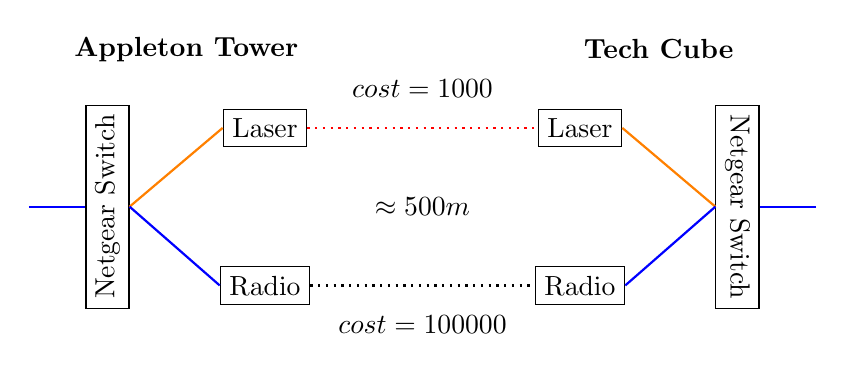
\begin{tikzpicture}
    \node at (1,2) {\textbf{Appleton Tower}};
    \node at (7,2) {\textbf{Tech Cube}};
    \cfdesign
  \end{tikzpicture}
  \caption{CableFree Link Design}
  \label{fig:cablefree-link}
\end{figure}

There were, however, several problems with this design. The less
serious was that this design was hardly appropriate for the local
environment. We already had a significant amount of radio equipment at
both sites -- including a radio link between them -- so an extra radio
link was superfluous. The radios specified by the vendor were low-end
Mikrotik radios with panel antennae in a waterproof enclosure. This is
not to cast aspersions on Mikrotik equipment, indeed we make much use
of it and it is generally quite good for the price. However Cablefree
wished to sell this re-branded equipment at a significant markup.

\begin{wrapfigure}{r}{0.3\textwidth}
  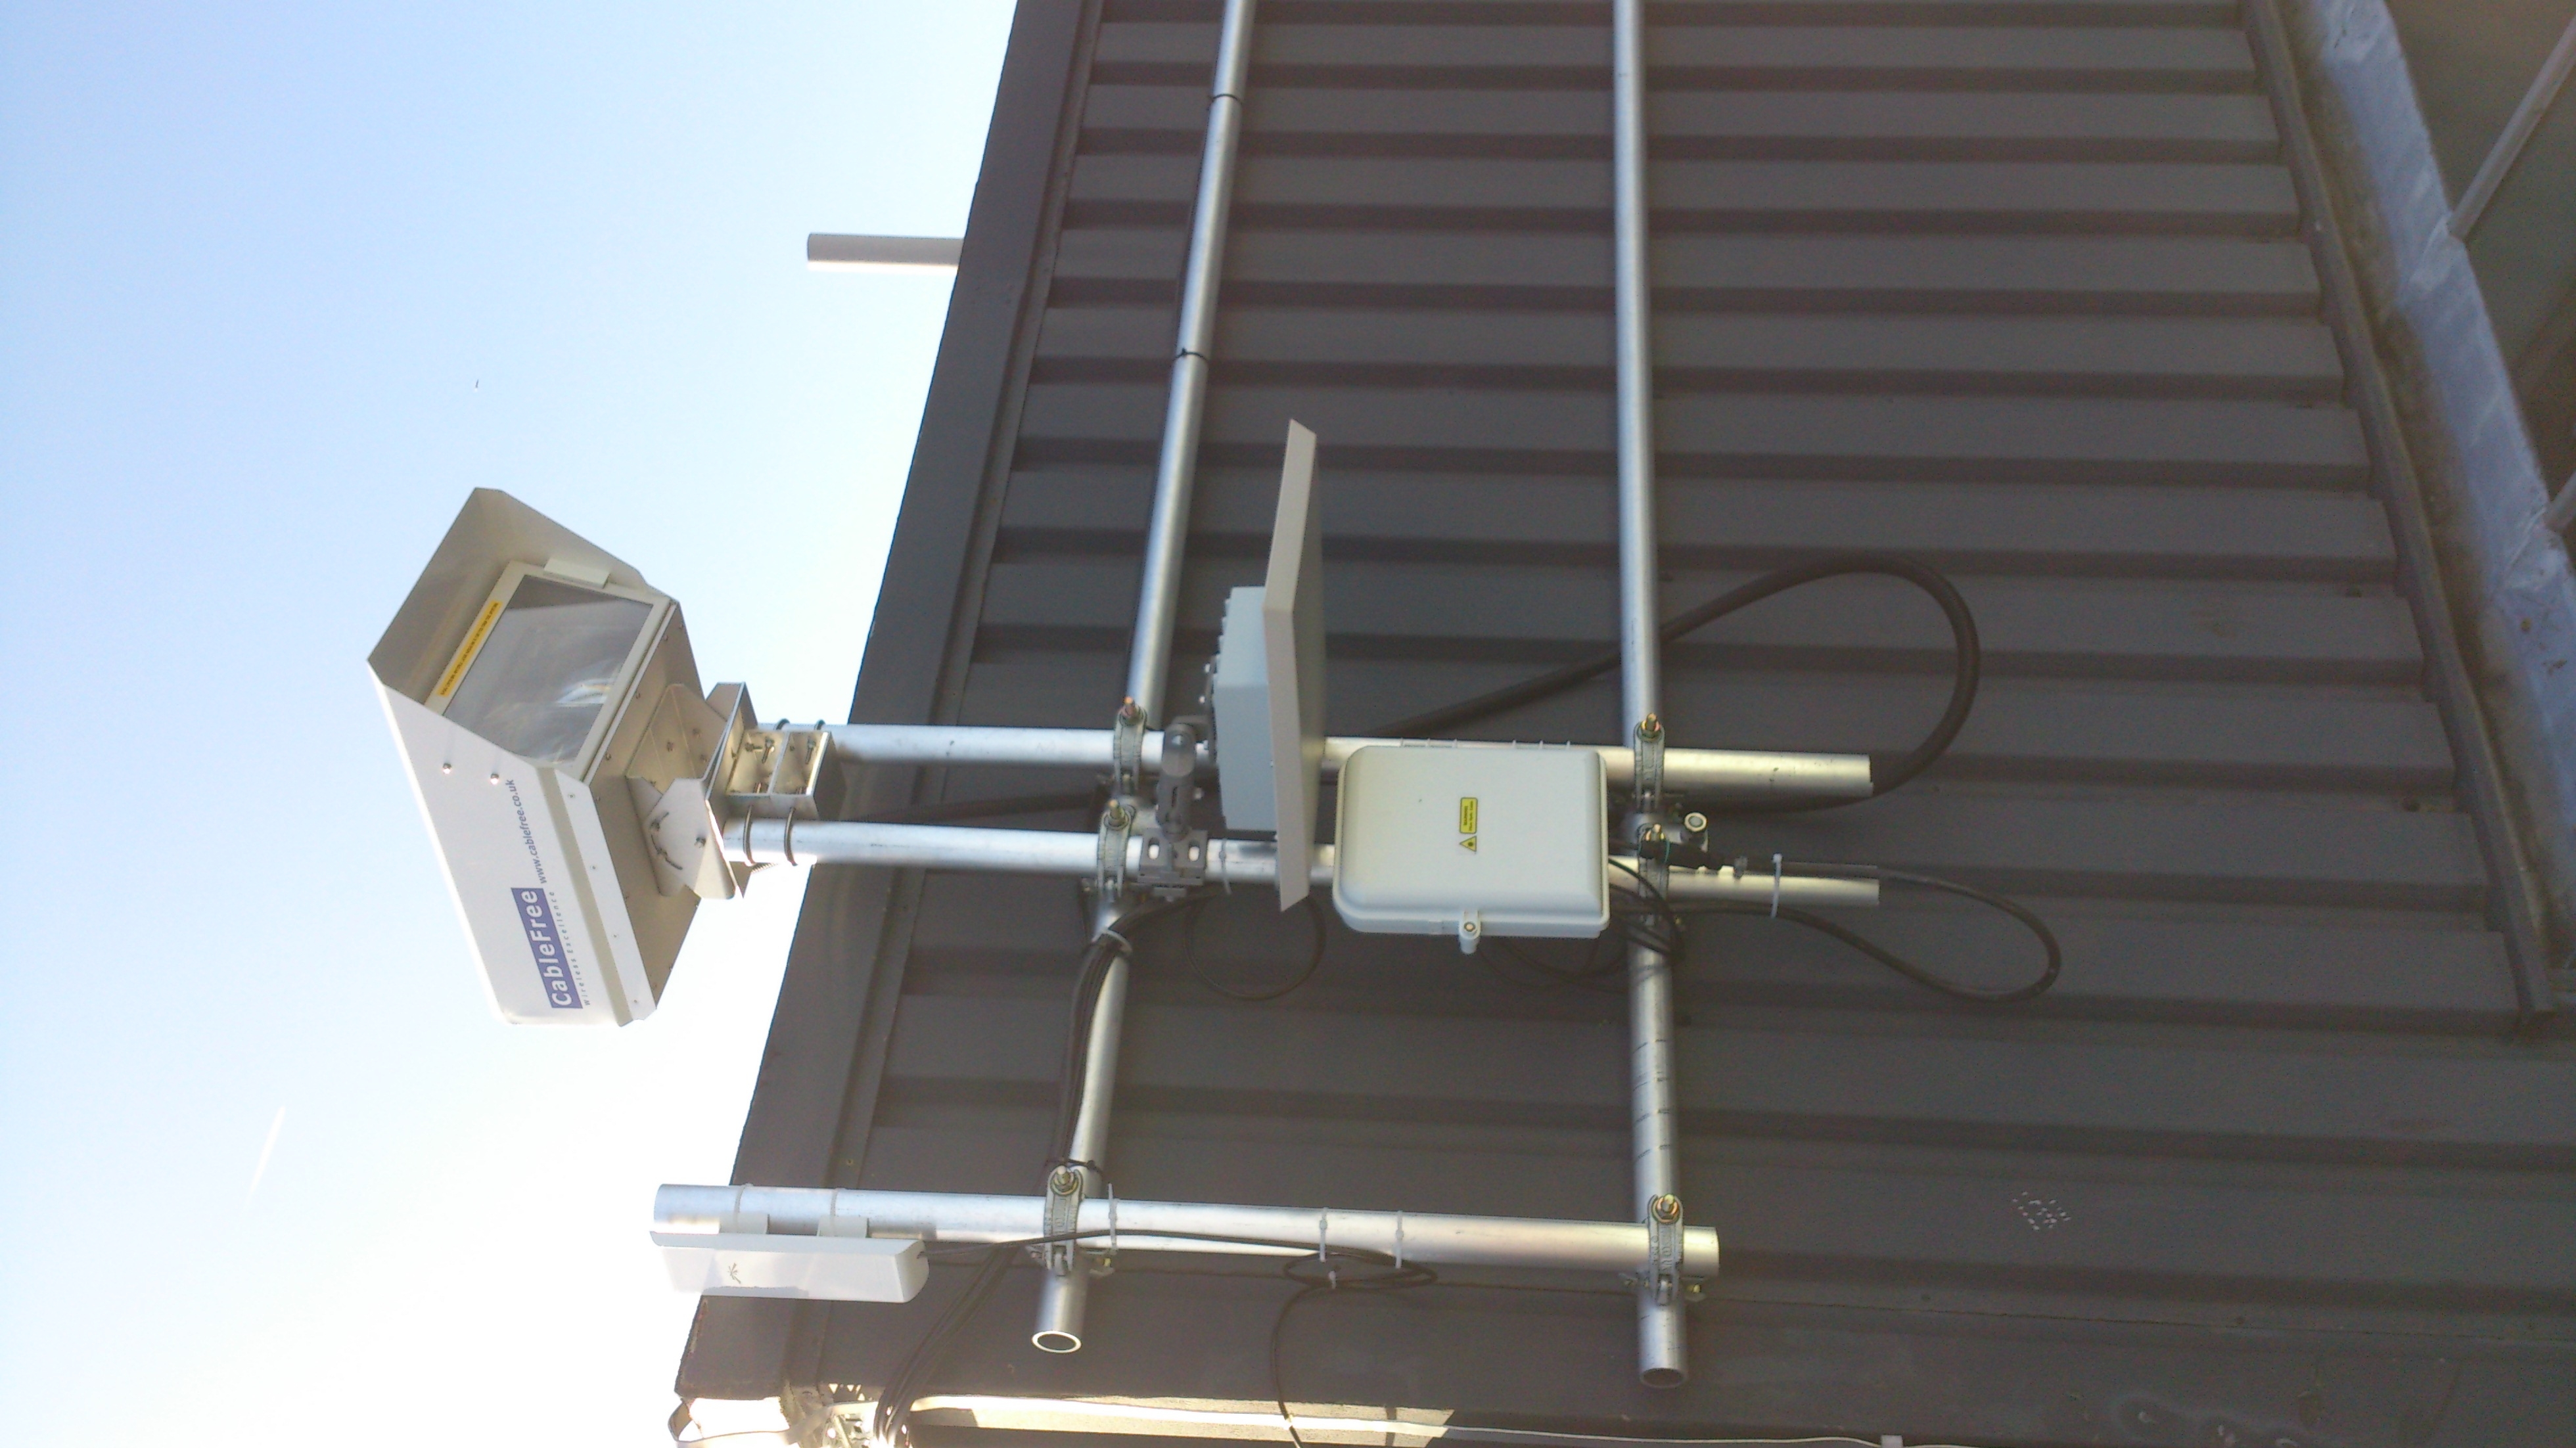
\includegraphics[angle=-90,width=0.3\textwidth]{also-faulty}
\end{wrapfigure}
Most amusingly, the mounting brackets supplied with the re-branded
Mikrotik radios were somewhat flimsy. It can get very windy at the top
of tall buildings in Edinburgh. Wind speeds can reach several times
more than at ground level. The installation is shown at right with the
mounting bracket having worked loose in high winds leaving the radio
pointing downwards.

We also had high end HP ProCurve J9050A switches at either end (loaned
by the School of Informatics), far more capable network elements than
the consumer-grade Netgear switches (see
Figure~\ref{fig:carrier-grade}) specified by the vendor. The
deficiencies of the Netgear switch are that it is not manageable via
telnet or ssh, which makes it very difficult to recover from outages
or erroneous configurations in a network of any size or complexity,
and more seriously, the cheap power adapter of the kind that are prone
to failure or simply disconnection due to the use of barrel
connectors. The power injector for the re-branded Mikrotik radio also
suffers from this deficiency (the white apparatus connected into the
switch in the photograph).

Unfortunately CableFree wished to sell a ``complete solution'' for us
to evaluate rather than an ``appropriate solution'' for our
circumstances and we succumbed to their hard-sell, ``complete'' with
sub-standard parts. We ultimately ended up operating the link by
connecting the vendor-supplied netgear switches to our HP switching
core and removing the vendor-supplied radio equipment entirely.
\begin{figure}
  \begin{center}
    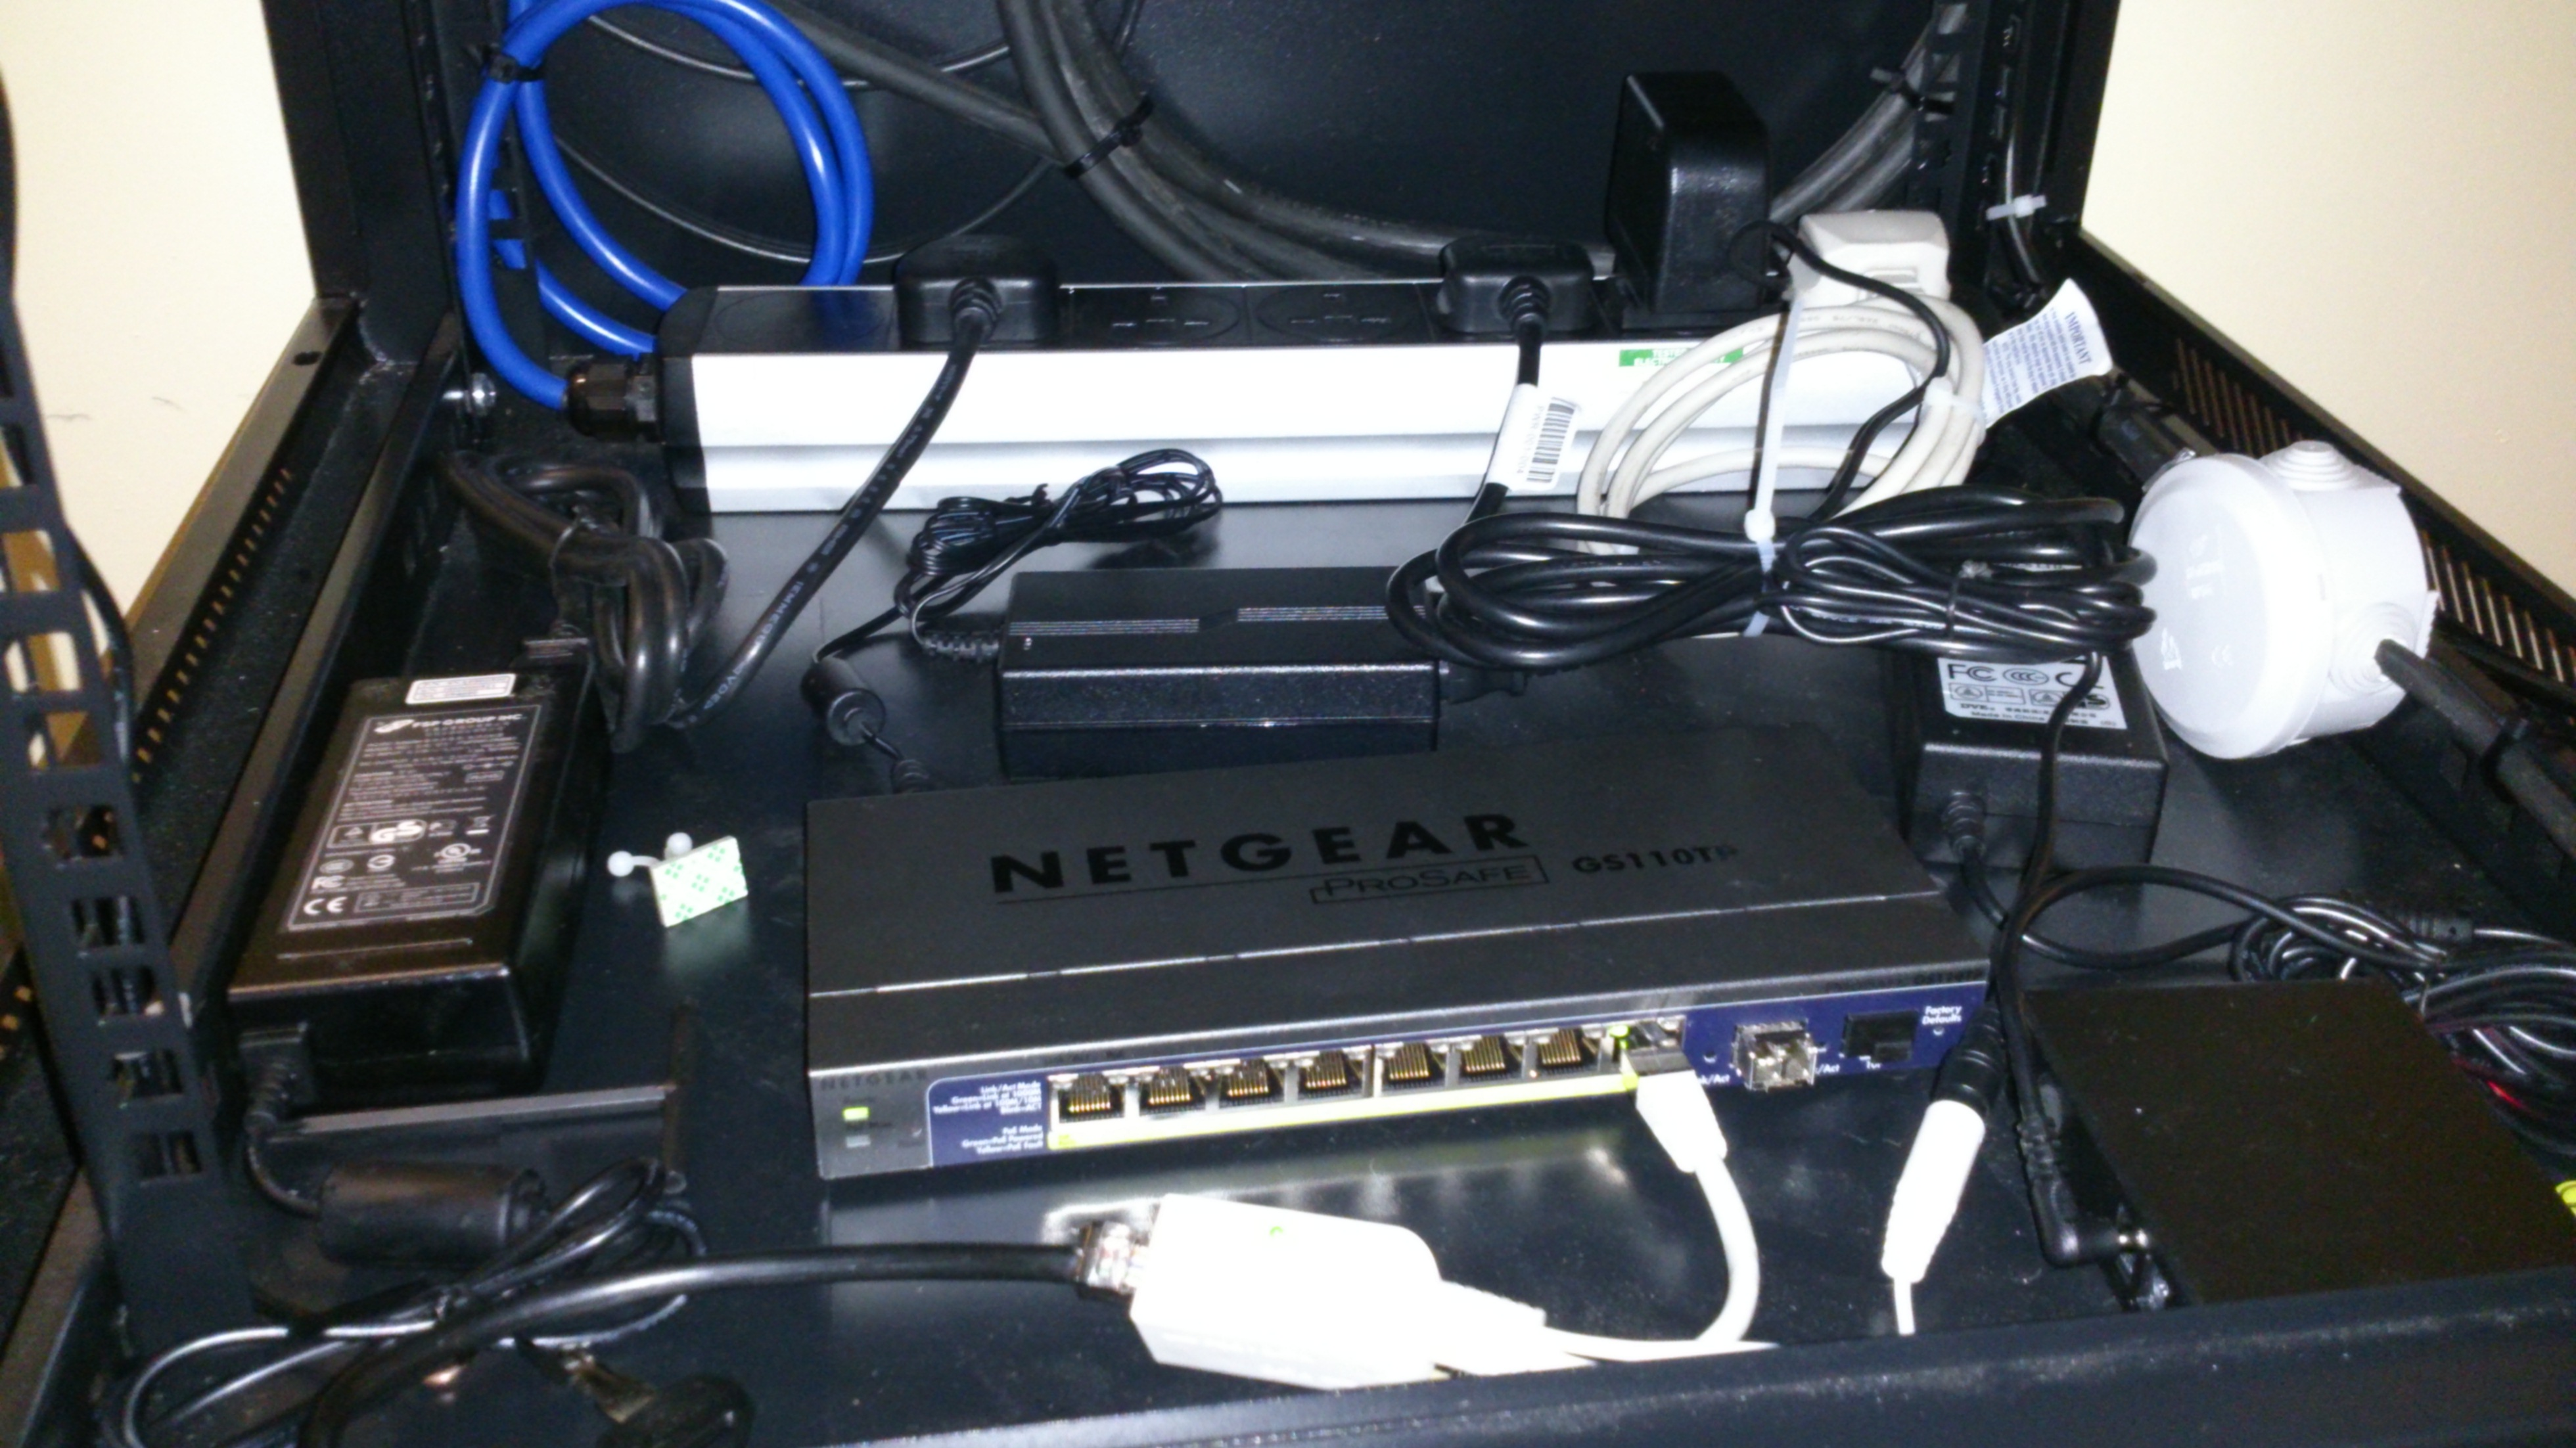
\includegraphics[width=0.5\textwidth]{carrier-grade}
  \end{center}
  \caption{A ``carrier-grade'' ethernet switch.}
  \label{fig:carrier-grade}
\end{figure}

The more serious deficiency with this design is the use of the
spanning-tree protocol. We will have more to say about the detail of
this below, but in brief, the mechanism is unstable in marginal
conditions. If the weather is clear or if the weather is very foggy,
the link operates as designed. However in the region between clear and
very foggy, the path is liable to rapidly change between the (possibly
unuseable) optical link and the radio link. Evidence for this is
anectodal due to the impossibility of properly instrumenting the
optical equipment, of which also more below.
\clearpage
\subsection{Fittings}
\label{sec:fittings}

\begin{wrapfigure}{r}{0.3\textwidth}
  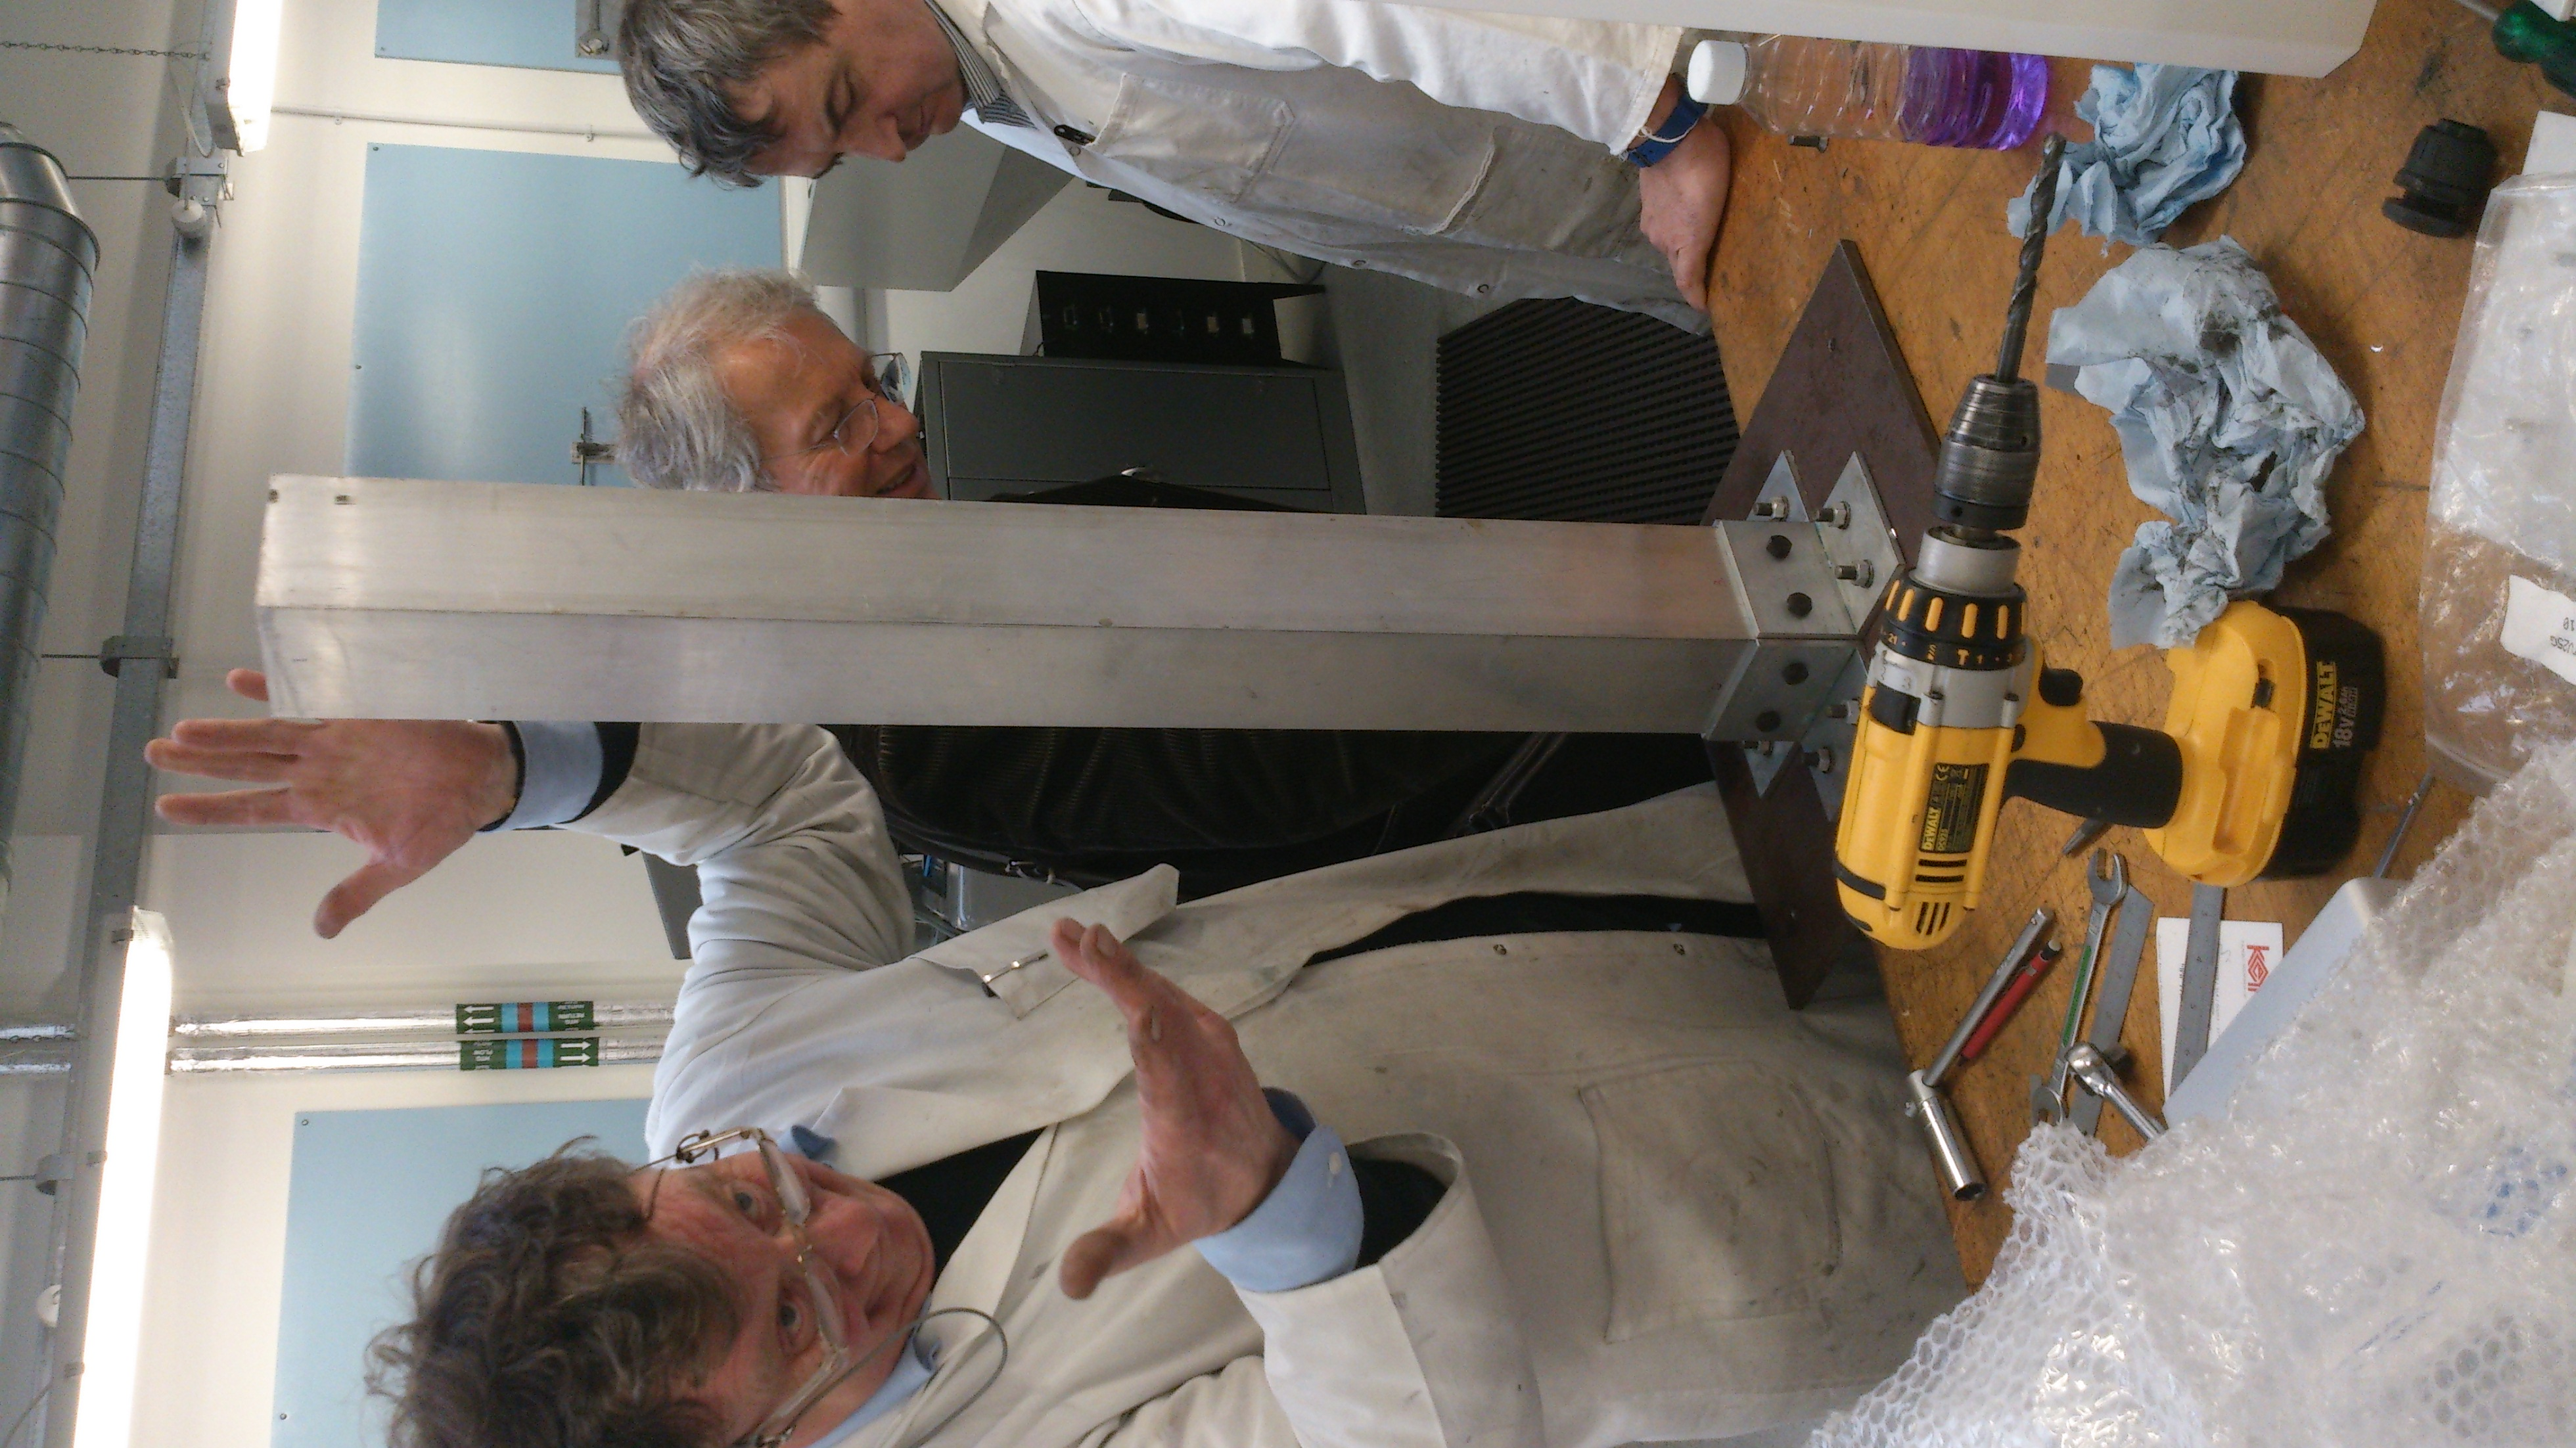
\includegraphics[angle=-90,width=0.3\textwidth]{tada}
\end{wrapfigure}
Story about trials and tribulations of getting them mounted...

And also how they had to have the glass screwed down because it came
off very easily...

\begin{figure}[h]
  \begin{center}
    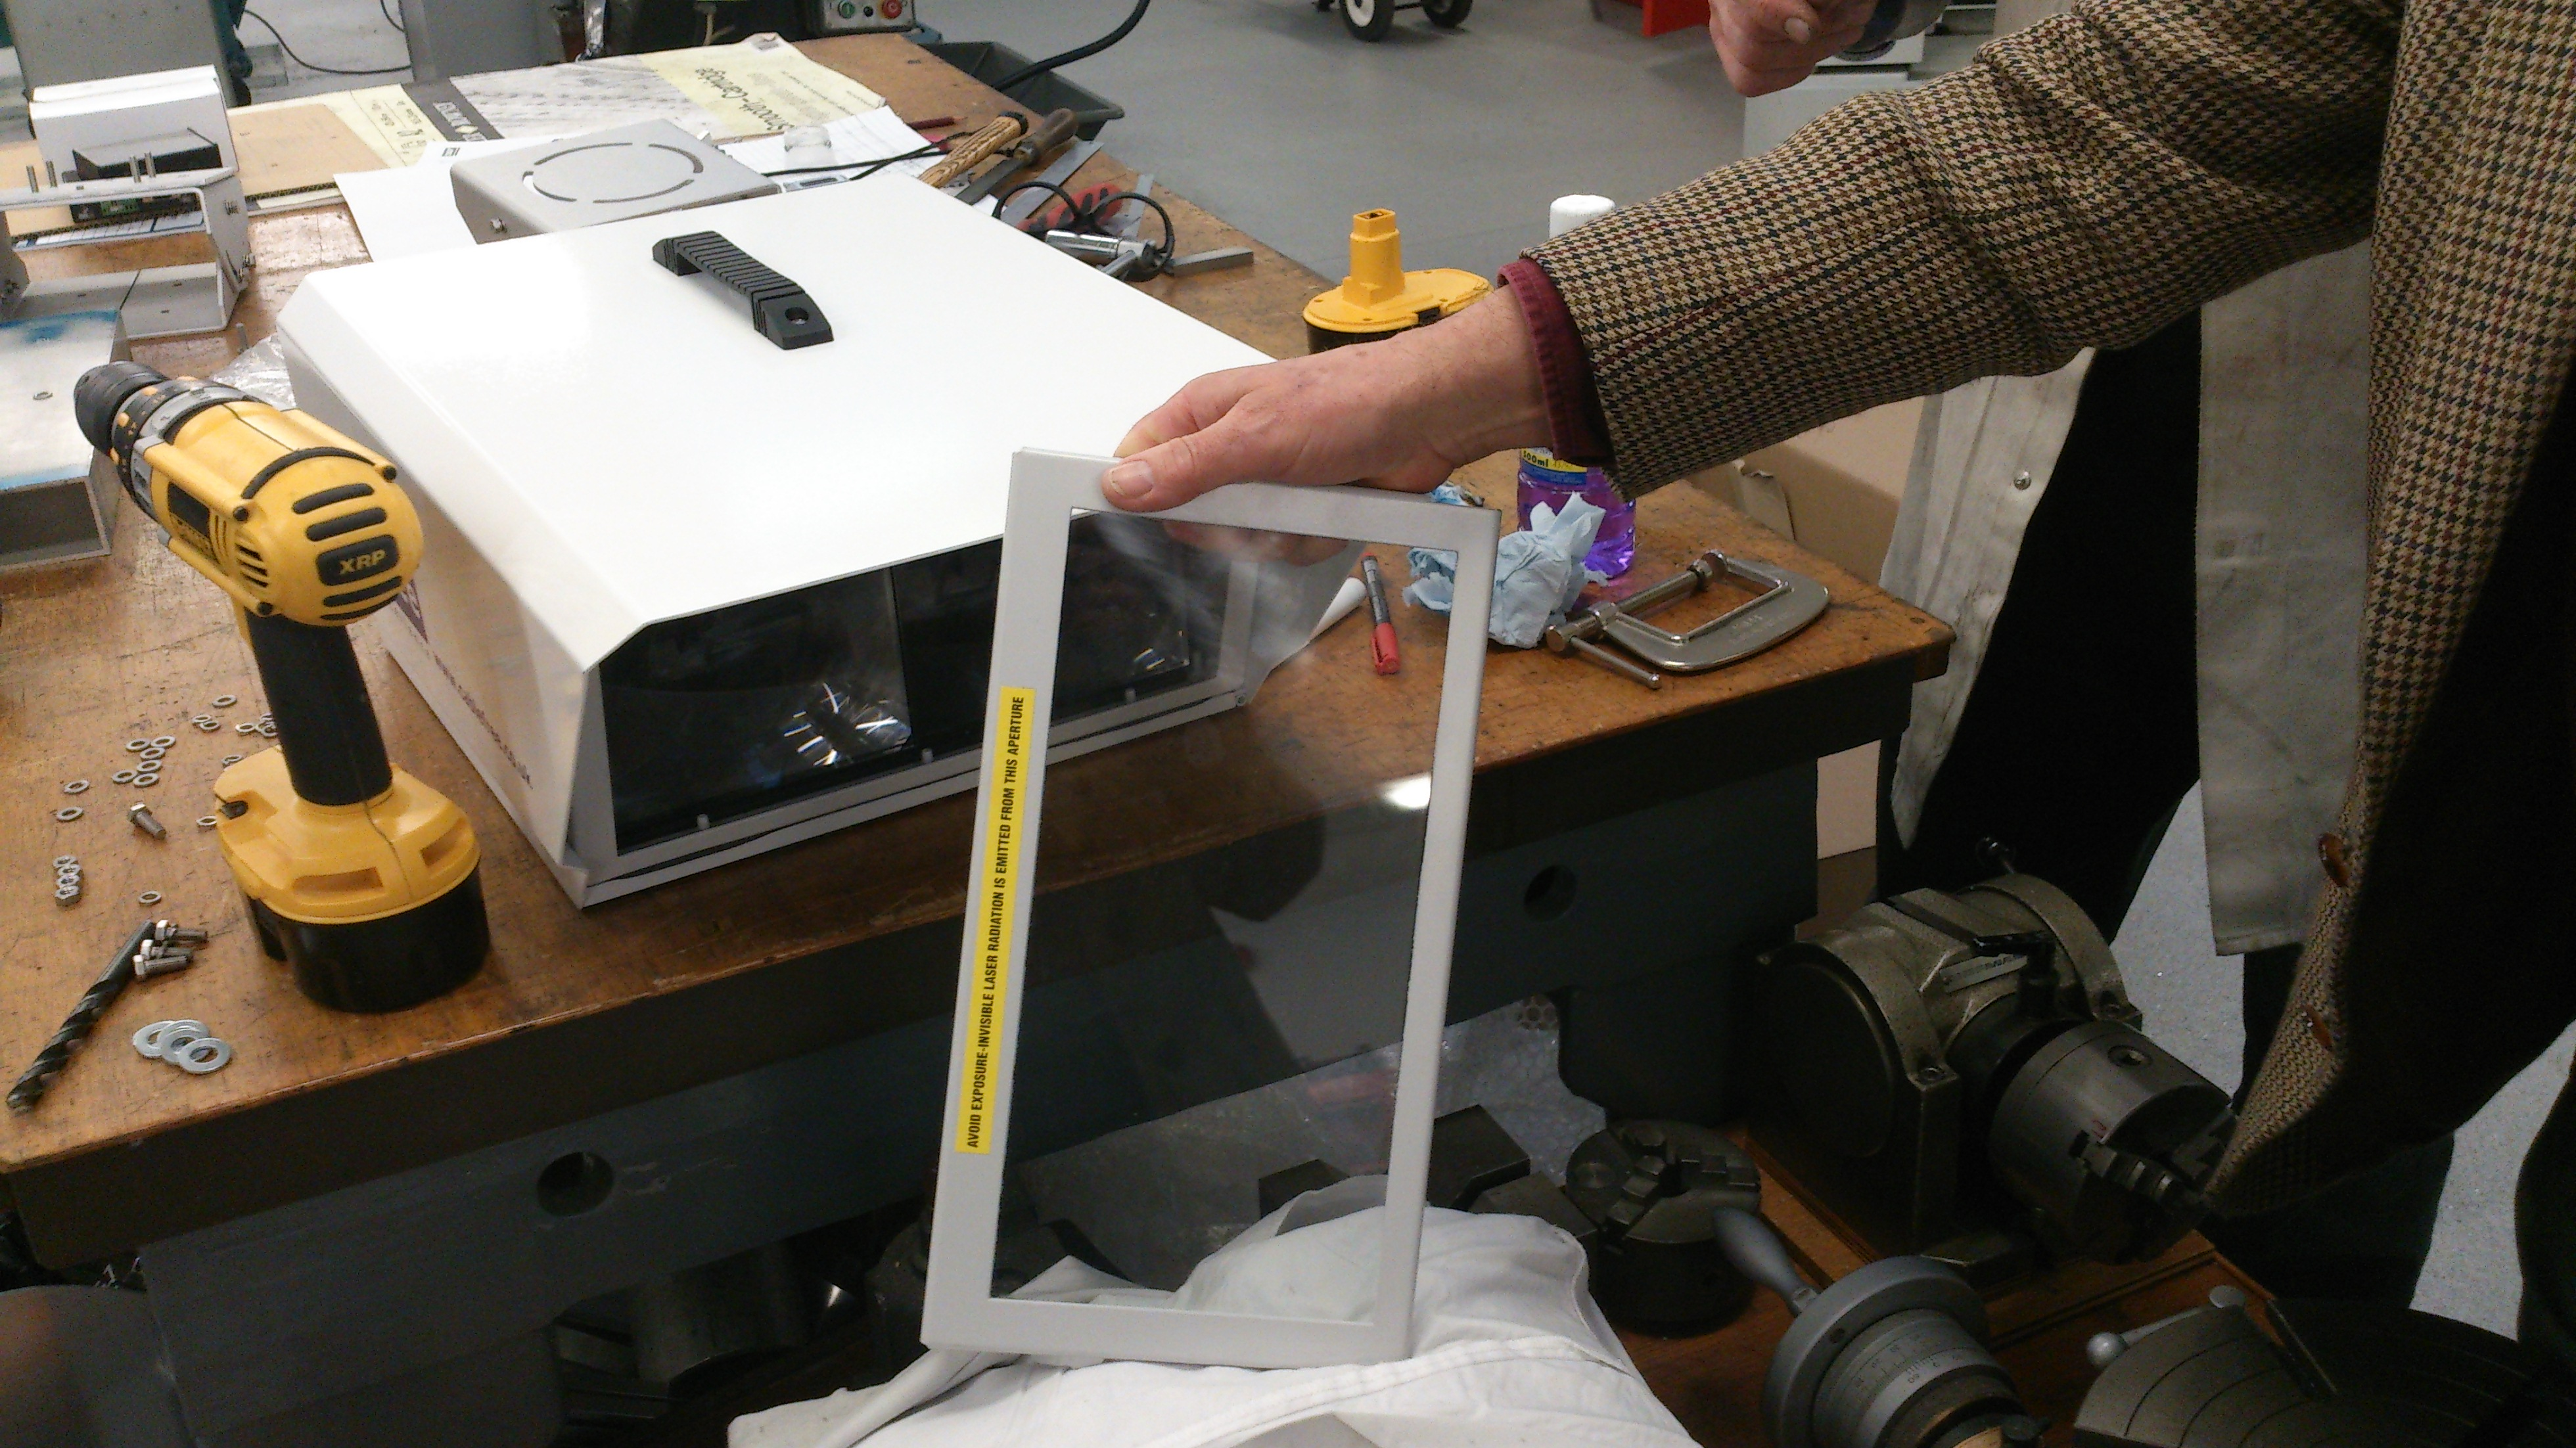
\includegraphics[width=0.5\textwidth]{faulty}
  \end{center}
\end{figure}

Not to mention the ``carrier grade'' netgear switch
\begin{figure}[h]
  \begin{center}
    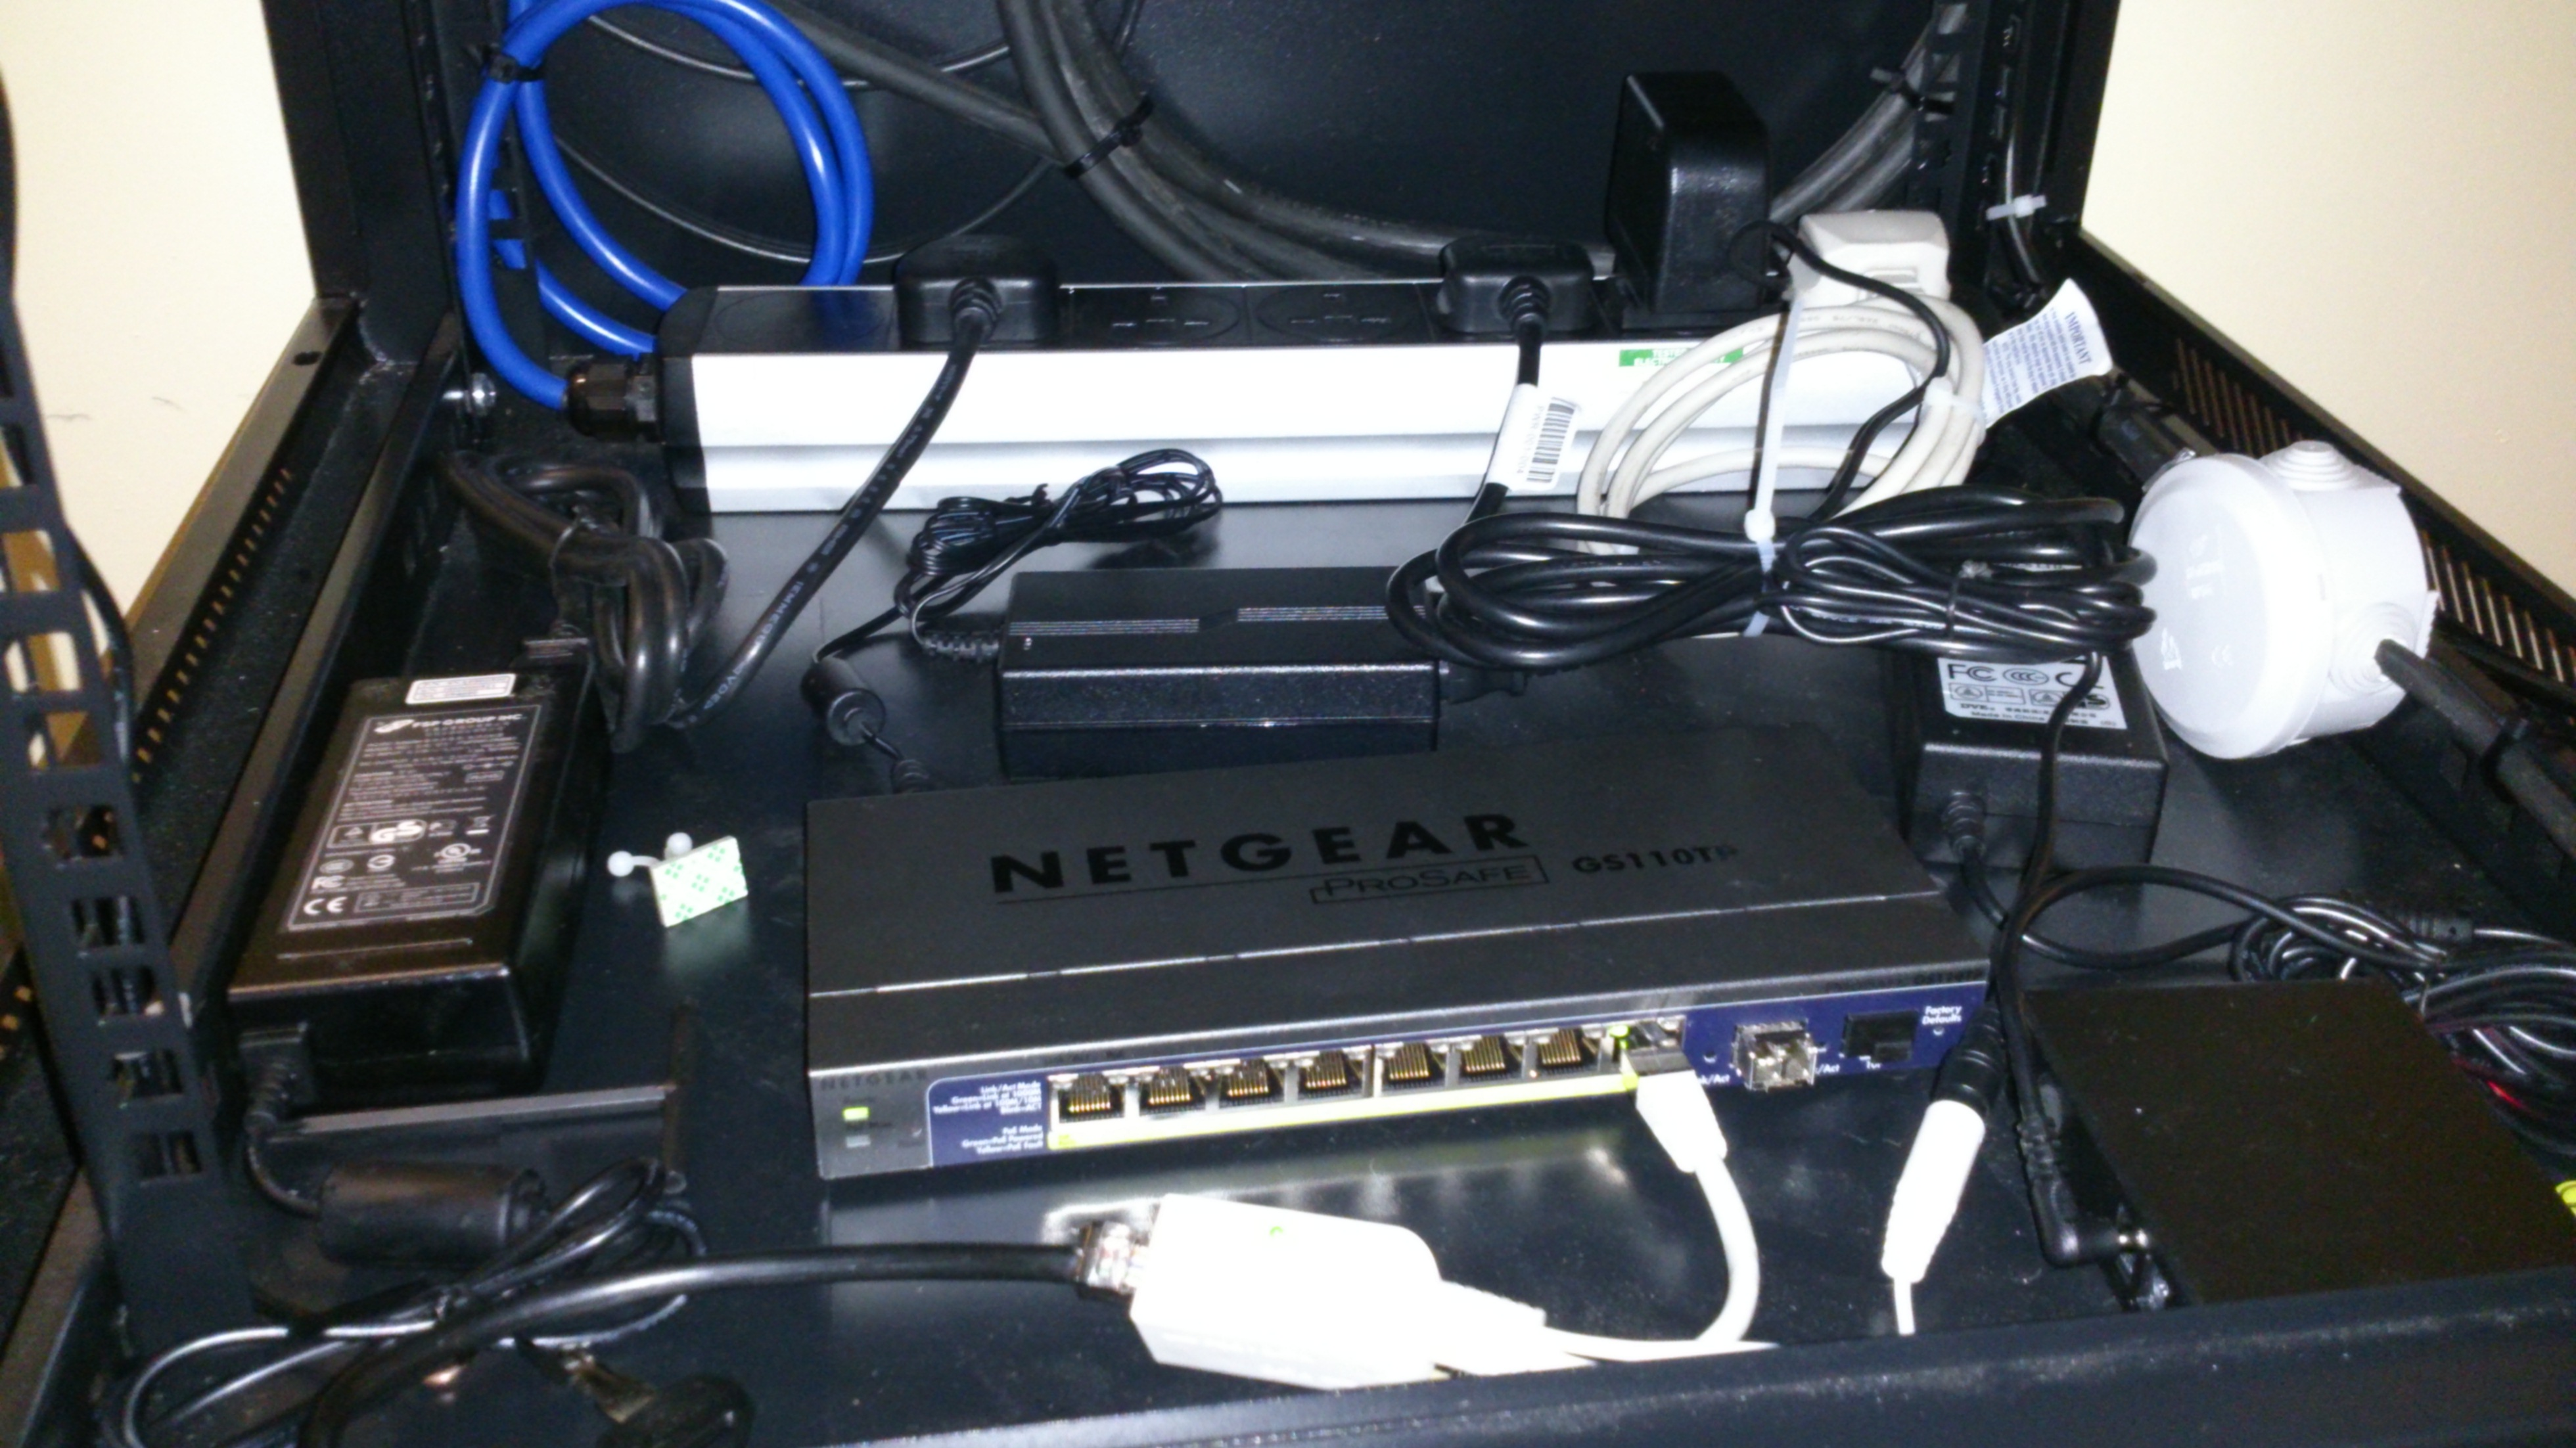
\includegraphics[width=0.5\textwidth]{carrier-grade}
  \end{center}
\end{figure}

And the feeble mounting brackets on the overpriced radio back-up link.
\begin{figure}[h]
  \begin{center}
    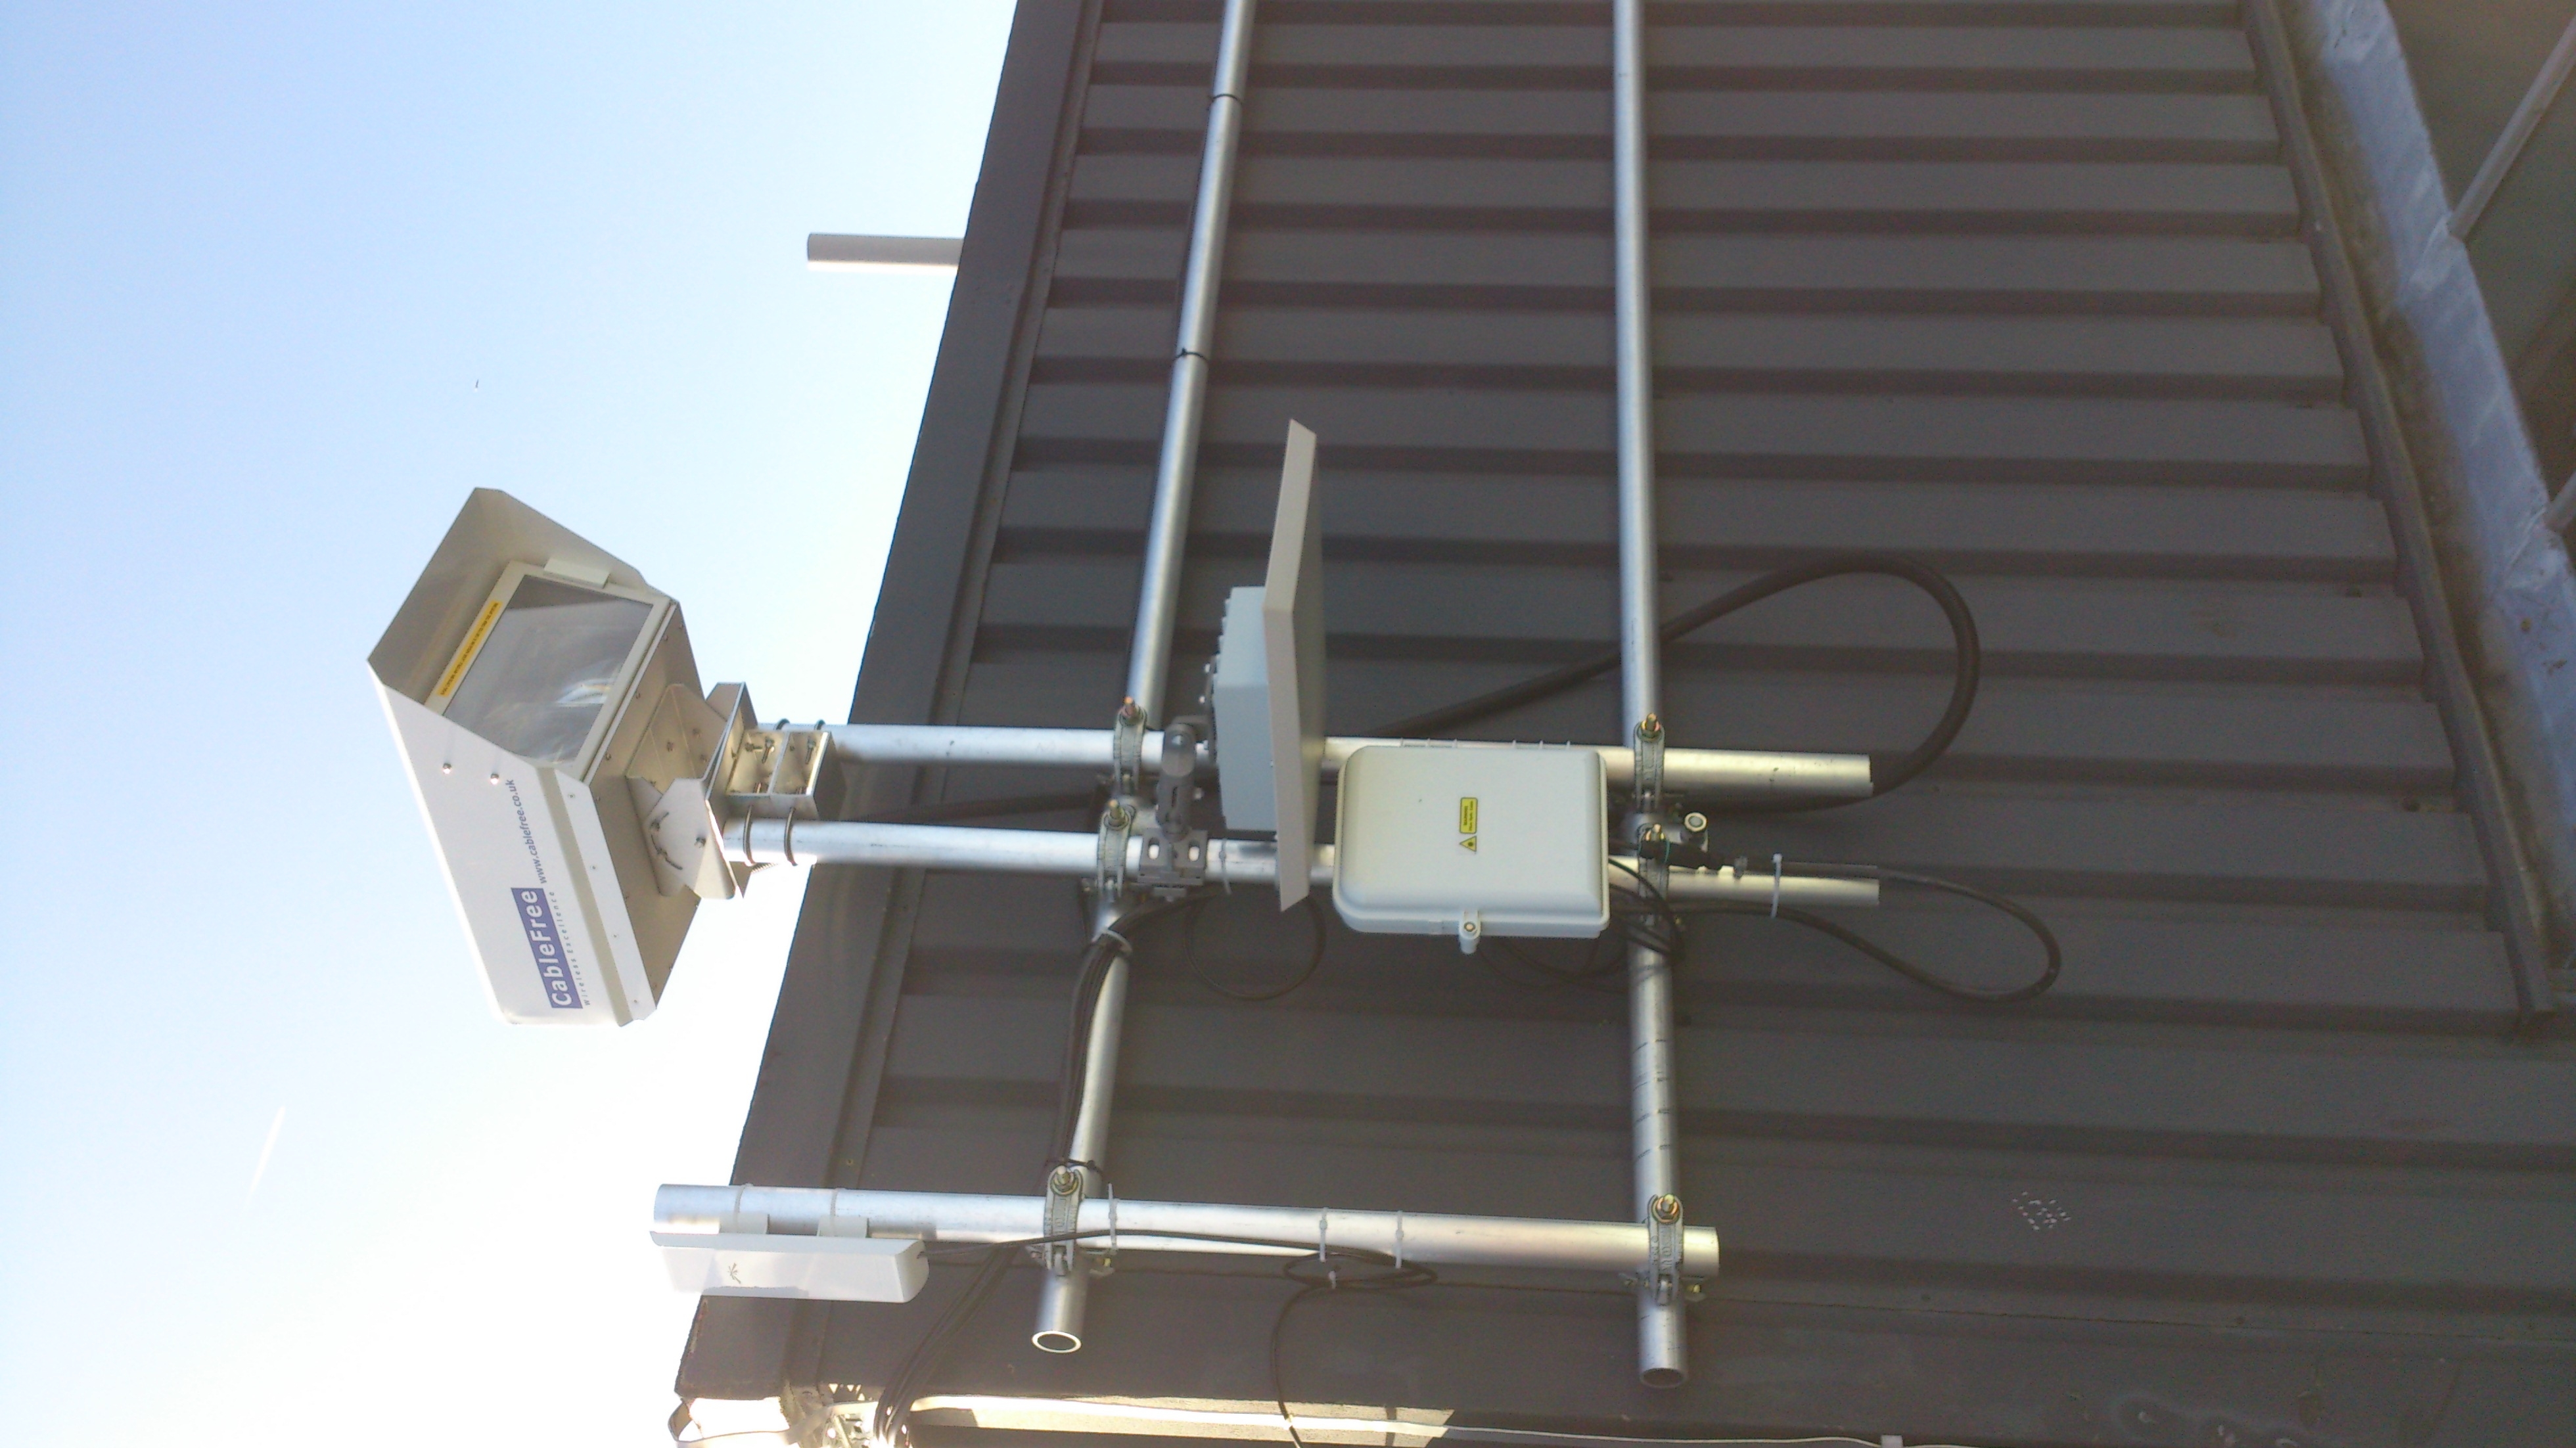
\includegraphics[angle=-90,width=0.5\textwidth]{also-faulty}
  \end{center}
\end{figure}

%%% Local Variables:
%%% mode: latex
%%% TeX-master: "scotgov-report"
%%% End:
